\documentclass[a4paper,11pt]{article}
\usepackage[a4paper,margin=1in,footskip=0.25in]{geometry}
\usepackage[utf8]{inputenc}

% science
\usepackage{amsmath}
\usepackage{array}
\usepackage{siunitx}

% layout
\usepackage{float}
\usepackage{parskip}
\usepackage{graphicx}
\usepackage{circuitikz}
\usepackage{longtable}
\usepackage{hyperref}


% referencing
\usepackage[style=apa]{biblatex}
\addbibresource{ratio.bib}
\usepackage{hyperref}

% table centering
\renewcommand{\arraystretch}{1.3}
\newcolumntype{P}[1]{>{\raggedright\arraybackslash}p{#1}}
\newcommand{\tptt}{$\times\,$}

% figures labelings
\usepackage{chngcntr}
\counterwithin{figure}{section}

\usepackage{caption}
\usepackage{subcaption}
\usepackage{wrapfig}

\title{Estimating the goodness of products based on its internet likes and dislikes using Bayesian statistics}

\author{}
\date{\vspace{-8ex}}

\begin{document}

\maketitle

\section{Introduction}

\begin{wrapfigure}{r}{0.4\textwidth}
    \centering
    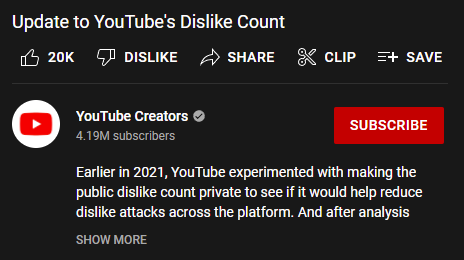
\includegraphics[width=0.45\textwidth]{assets/intro.png}
    \caption{Hidden Dislikes}
    \label{fig:hidden}
\end{wrapfigure}

This topic is chosen out of my curiously towards a very insignificant change. For I often procrastinate when doing my homework, I stumbled across a post on an online forum announcing the the popular internet video sharing platform of YouTube of removing their dislike counts (shown in Figure \ref{fig:hidden}). As usual, I dug into the comment section and all the various complaints that one will expect on the internet --- how YouTube is on a decline towards big companies, that this is the stupidest decision an internet company has made, all but one has caught my eye:

\begin{quote}
    Dislike counts were necessary to spot clickbait, scams, fake tutorials, blatant misinformation, etc. --- Element 115 (internet user)
\end{quote}

The usage of likes and dislikes as a metric of legibility and quality is something that I knew and used extensively, mostly in saving my precious time in judging the qualities of the a series of maths videos made for the trend ``Summer of Math Exposition'' consisting of mostly amateur video makers. While the removal of the dislike counts demonstrated on how reliant I was on a simple number, it also led me to wonder of my technique in judging the quality of a video.
% think about


\section{Ratios}

\end{document}
